\documentclass[fleqn]{article}
\usepackage[nodisplayskipstretch]{setspace}
\usepackage{amsmath, nccmath, bm}
\usepackage{amssymb}
\usepackage{enumitem}
\usepackage{etoolbox}
\usepackage{graphicx}
\usepackage{float}
\usepackage{changepage}
\usepackage{environ,capt-of}

\let\oldfigure\figure% Store original figure float environment
\let\endoldfigure\endfigure
\RenewEnviron{figure}[1][H]{% Update figure environment
  %\par\vspace{\intextsep}% Assume in-text placement, so insert appropriate vertical spacing
  \noindent
  % \patchcmd{<cmd>}{<search>}{<replace>}{<success>}{<failure>}
  \patchcmd{\BODY}{\caption}{\captionof{figure}}{}{}% Replace \caption with \captionof{figure} inside \BODY
  % Set "figure"
  \begin{minipage}{\linewidth}
    \BODY
  \end{minipage}
  %\par\vspace{\intextsep}% Assume in-text placement, so insert appropriate vertical spacing
}

\newcommand{\zerodisplayskip}{
	\setlength{\abovedisplayskip}{0pt}%
	\setlength{\belowdisplayskip}{0pt}%
	\setlength{\abovedisplayshortskip}{0pt}%
	\setlength{\belowdisplayshortskip}{0pt}%
	\setlength{\mathindent}{0pt}}
	
\title{Homework 3}
\author{Owen Sowatzke}
\date{March 13, 2024}

\begin{document}

	\offinterlineskip
	\setlength{\lineskip}{12pt}
	\zerodisplayskip
	\maketitle
	
	\begin{enumerate}
		\item The exclusive-OR is the simplest problem that cannot be solved using a linear discriminant operating directly on the features. The points $k=1,3$ at $\mathbf{x} = [1,1]^T$ and $[-1,-1]^T$ are in the category $\omega_1$ (red in the figure), while $k=2,4$ at $\mathbf{x}=[1,-1]^T$ and $[-1,1]^T$ are in $\omega_2$ (black in the figure). Following the approach of Support Vector Machines, we preprocess the features to map them to a higher dimension space where they can be linearly separated. While many $\varphi$-functions could be used, here we use the simplest expansion up to second order: $1, \sqrt{2}x_1, \sqrt{2}x_2, \sqrt{2}x_1x_2, x_1^2$ and $x_2^2$, where the $\sqrt{2}$ is convenient for normalization. Using the support vector machine formulation, show that the optimum discriminant is $g(\mathbf{x}) = g(x_1,x_2) = x_1 * x_2$.
		
		\begin{figure}[H]
			\centerline{\fbox{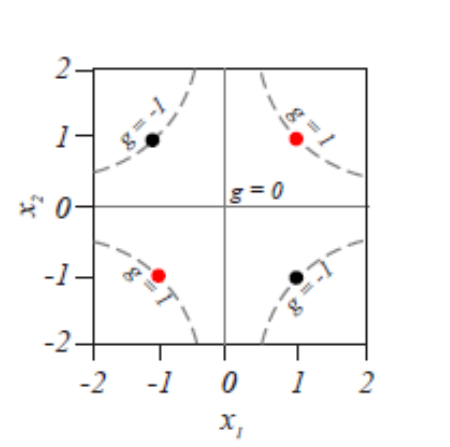
\includegraphics[width=0.4\textwidth]{exclusive_or.png}}}
			\caption{Exclusive-OR Problem}
			\label{exclusive_or}
		\end{figure}
	\end{enumerate}
\end{document}